              
% --------------------------------------------------------------
% This is all preamble stuff that you don't have to worry about.
% Head down to where it says "Start here"
% --------------------------------------------------------------
 
\documentclass[11pt]{article}
\usepackage[utf8]{inputenc} 
\usepackage[margin=1in]{geometry}
\usepackage{graphicx}
\usepackage{float}
\usepackage{hyperref} 
\usepackage{amsmath,amsthm,amssymb}
\usepackage[table]{xcolor}
 
\newcommand{\N}{\mathbb{N}}
\newcommand{\Z}{\mathbb{Z}}
 
\newenvironment{theorem}[2][Theorem]{\begin{trivlist}
\item[\hskip \labelsep {\bfseries #1}\hskip \labelsep {\bfseries #2.}]}{\end{trivlist}}
\newenvironment{lemma}[2][Lemma]{\begin{trivlist}
\item[\hskip \labelsep {\bfseries #1}\hskip \labelsep {\bfseries #2.}]}{\end{trivlist}}
\newenvironment{exercise}[2][Exercise]{\begin{trivlist}
\item[\hskip \labelsep {\bfseries #1}\hskip \labelsep {\bfseries #2.}]}{\end{trivlist}}
\newenvironment{reflection}[2][Reflection]{\begin{trivlist}
\item[\hskip \labelsep {\bfseries #1}\hskip \labelsep {\bfseries #2.}]}{\end{trivlist}}
\newenvironment{proposition}[2][Proposition]{\begin{trivlist}
\item[\hskip \labelsep {\bfseries #1}\hskip \labelsep {\bfseries #2.}]}{\end{trivlist}}
\newenvironment{corollary}[2][Corollary]{\begin{trivlist}
\item[\hskip \labelsep {\bfseries #1}\hskip \labelsep {\bfseries #2.}]}{\end{trivlist}}
 
\begin{document}
 
% --------------------------------------------------------------
%                         Start here
% --------------------------------------------------------------
 
\setlength\parindent{0pt}
%\renewcommand{\qedsymbol}{\filledbox}
 
\title{Assignment 3: N-armed bandit problem}%replace X with the appropriate number
\author{Pierre Gérard (ULB)\\ %replace with your name
INFO-F-409 - Learning dynamics} %if necessary, replace with your course title
 
\maketitle

\section{N-Armed Bandit}

\subsection{Exercice 1}

\subsubsection{Average reward for each algorithm}

\begin{figure}[H]
   \centering
   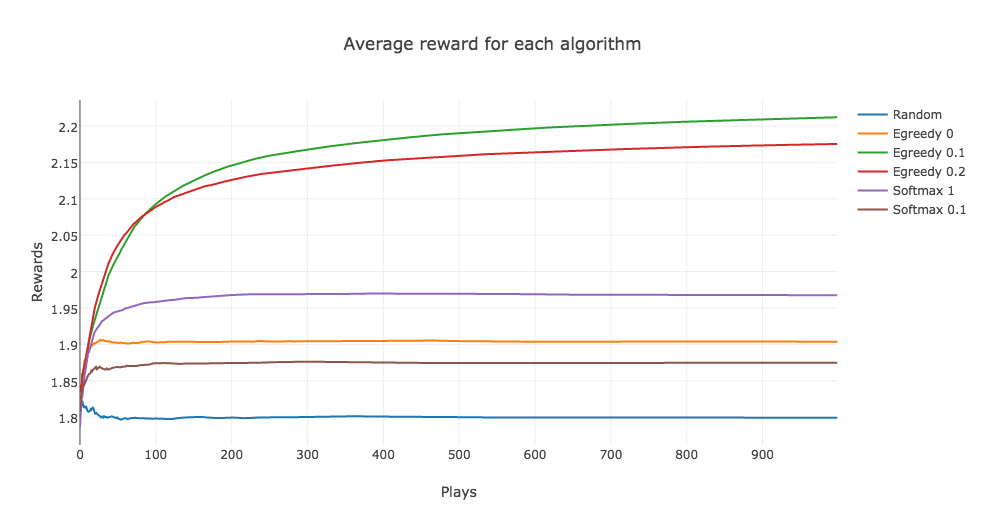
\includegraphics[width=0.8\textwidth]{img/1-1/reward.png}
\end{figure}

\subsubsection{Plot per arm}

\begin{figure}[H]
   \centering
   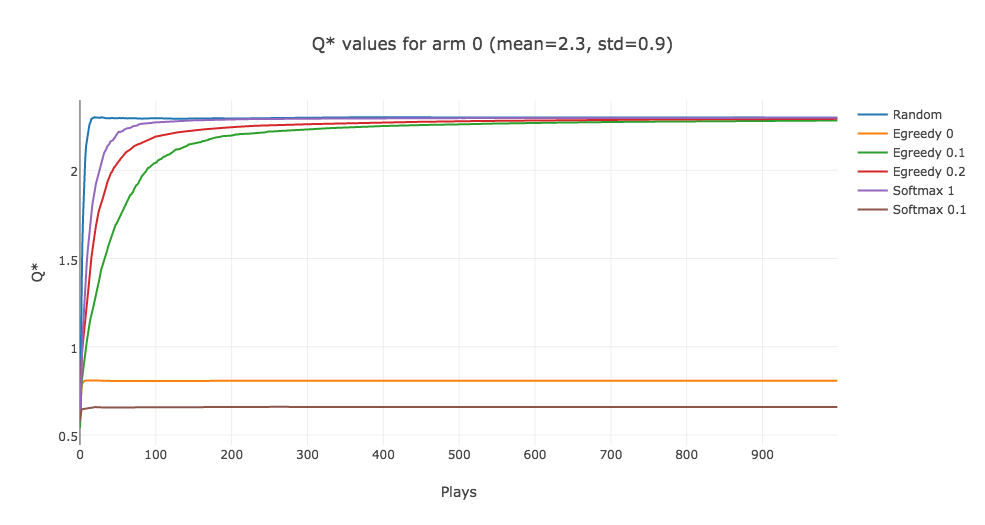
\includegraphics[width=0.7\textwidth]{img/1-1/q1.png}
\end{figure}

\begin{figure}[H]
   \centering
   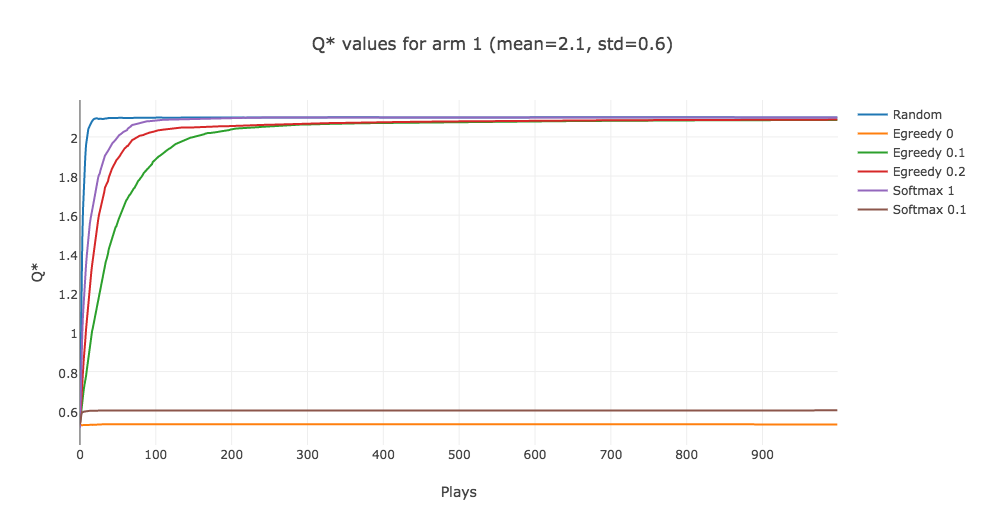
\includegraphics[width=0.7\textwidth]{img/1-1/q2.png}
\end{figure}

\begin{figure}[H]
   \centering
   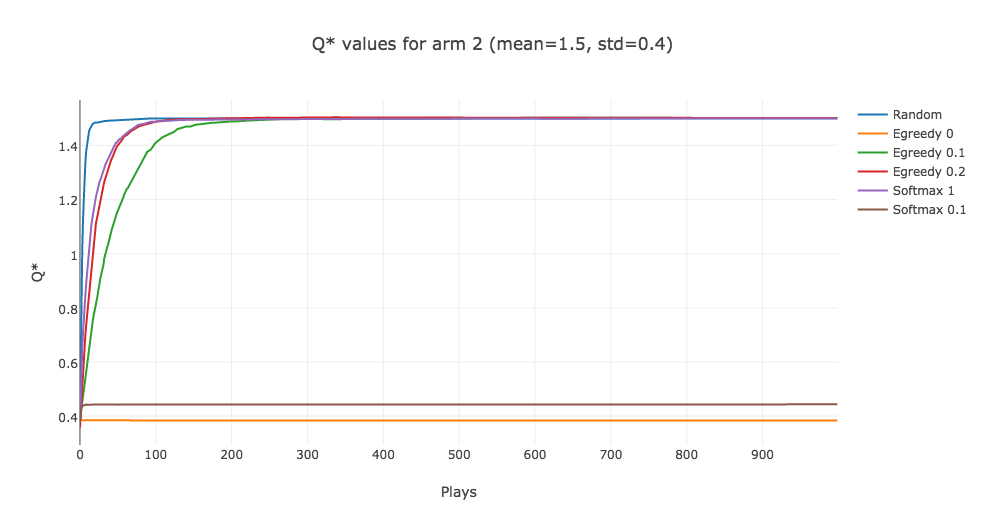
\includegraphics[width=0.7\textwidth]{img/1-1/q3.png}
\end{figure}


\begin{figure}[H]
   \centering
   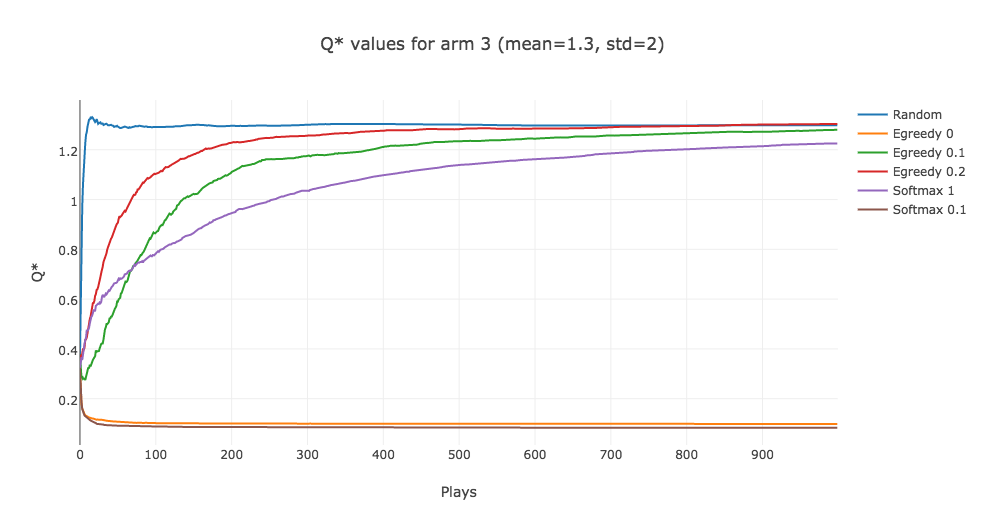
\includegraphics[width=0.7\textwidth]{img/1-1/q4.png}
\end{figure}


\subsubsection{Histogram}

\begin{figure}[H]
   \centering
   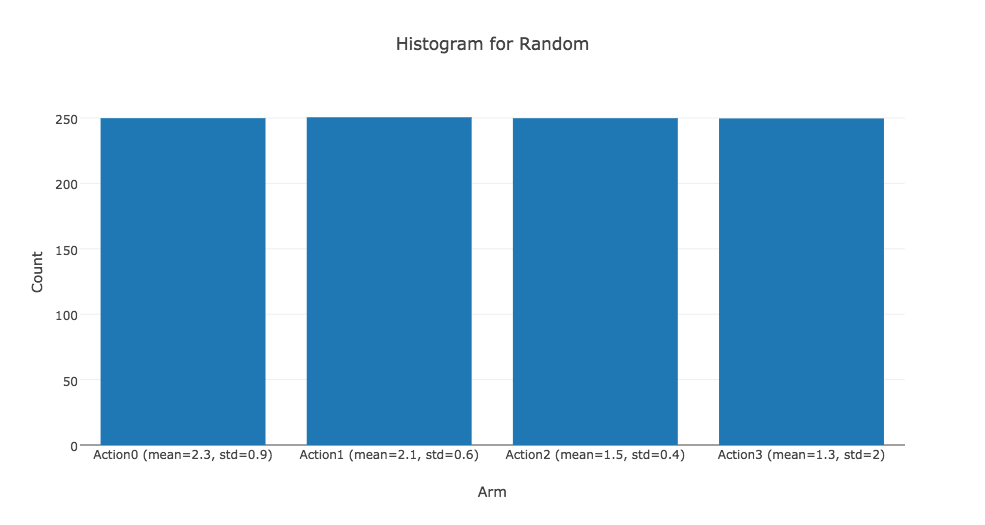
\includegraphics[width=0.7\textwidth]{img/1-1/h1.png}
\end{figure}

\begin{figure}[H]
   \centering
   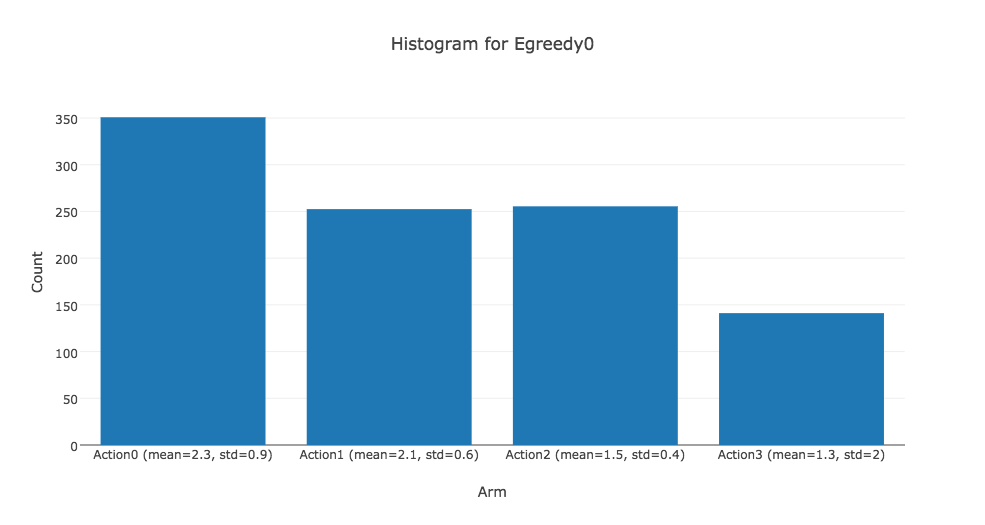
\includegraphics[width=0.7\textwidth]{img/1-1/h2.png}
\end{figure}

\begin{figure}[H]
   \centering
   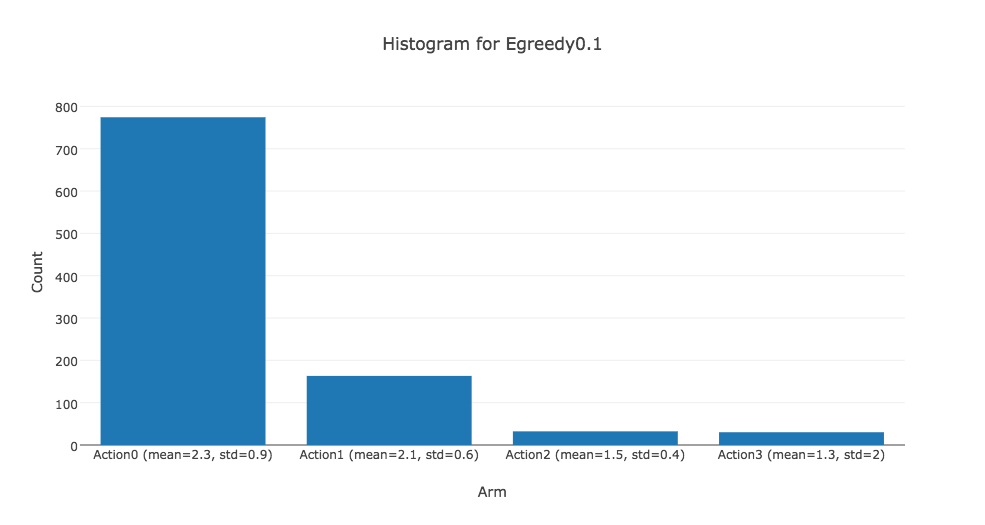
\includegraphics[width=0.7\textwidth]{img/1-1/h3.png}
\end{figure}

\begin{figure}[H]
   \centering
   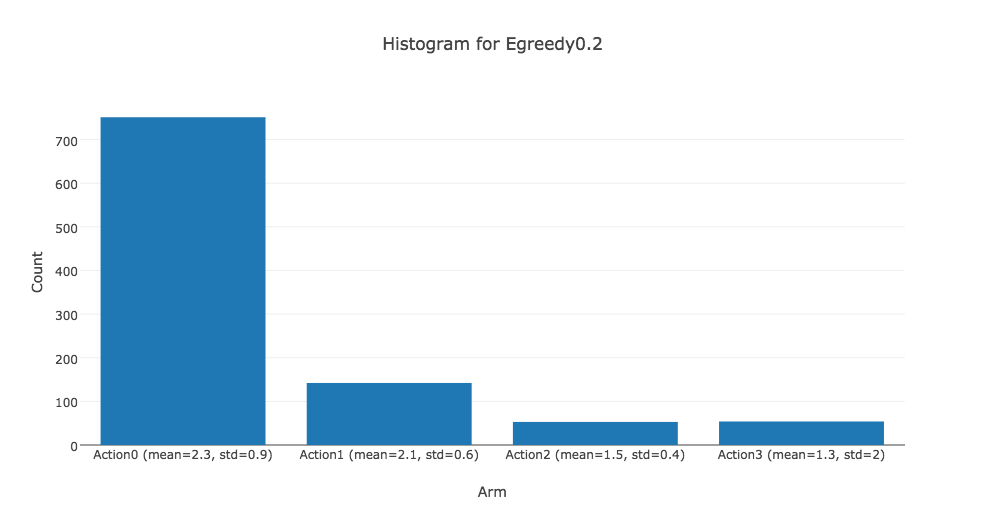
\includegraphics[width=0.7\textwidth]{img/1-1/h4.png}
\end{figure}

\begin{figure}[H]
   \centering
   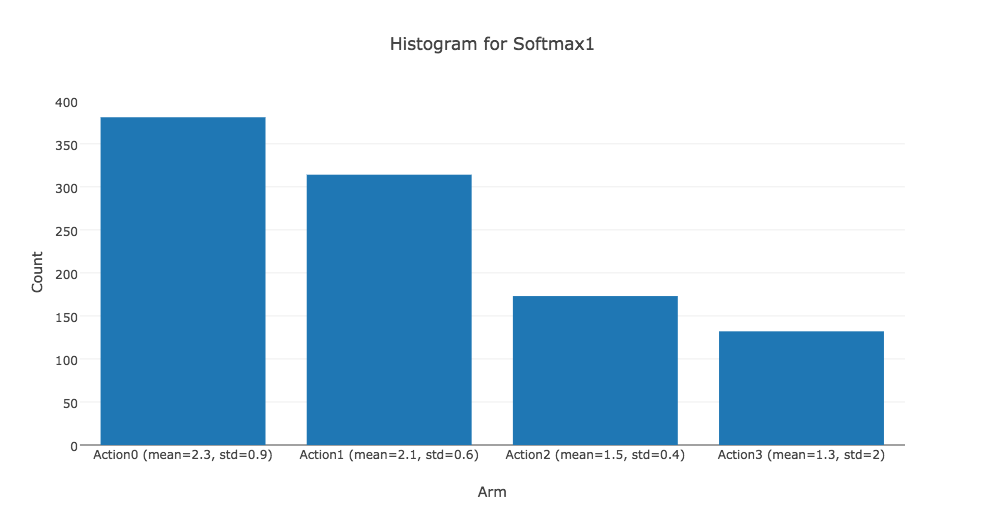
\includegraphics[width=0.7\textwidth]{img/1-1/h5.png}
\end{figure}

\begin{figure}[H]
   \centering
   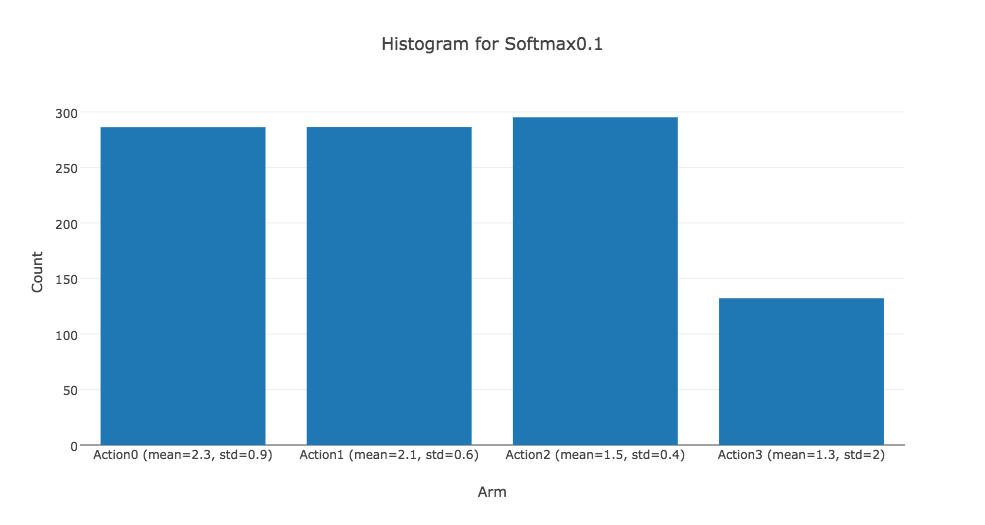
\includegraphics[width=0.7\textwidth]{img/1-1/h6.png}
\end{figure}


\subsubsection{Results}

\subsection{Exercice 2}


\subsubsection{Average reward for each algorithm}

\begin{figure}[H]
   \centering
   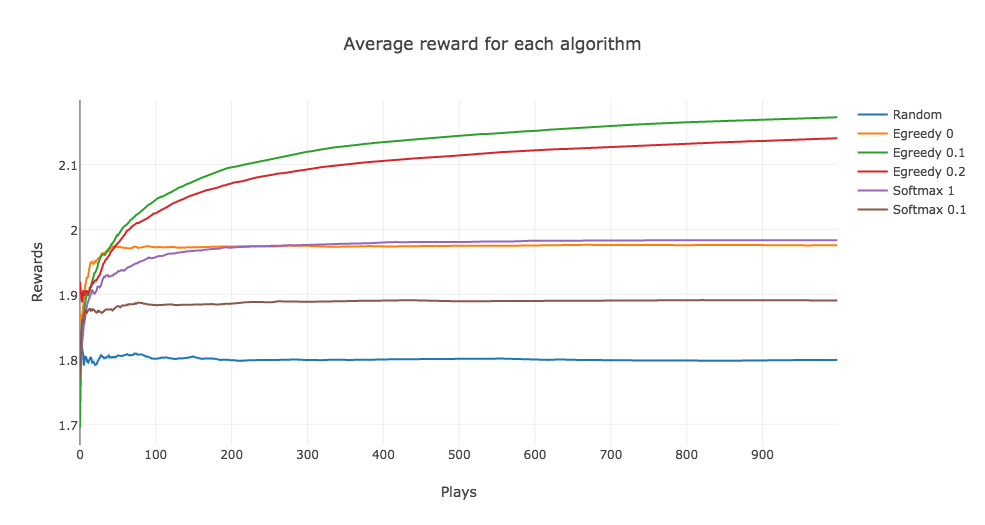
\includegraphics[width=0.8\textwidth]{img/1-2/reward.png}
\end{figure}

\subsubsection{Plot per arm}

\begin{figure}[H]
   \centering
   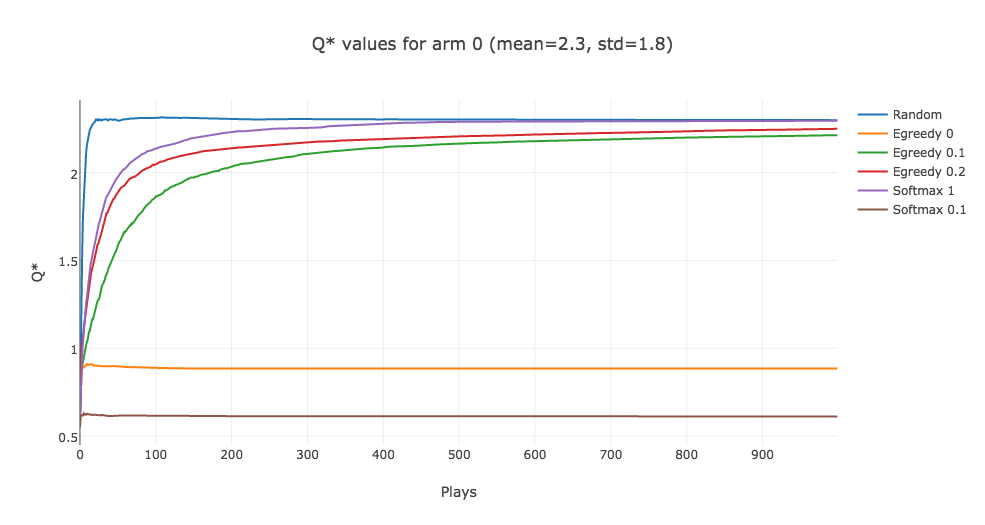
\includegraphics[width=0.7\textwidth]{img/1-2/q1.png}
\end{figure}

\begin{figure}[H]
   \centering
   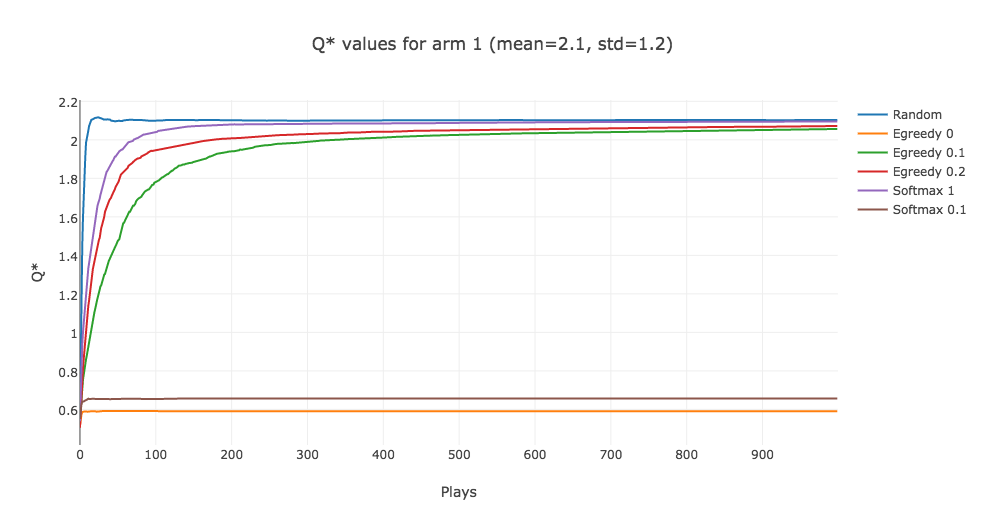
\includegraphics[width=0.7\textwidth]{img/1-2/q2.png}
\end{figure}

\begin{figure}[H]
   \centering
   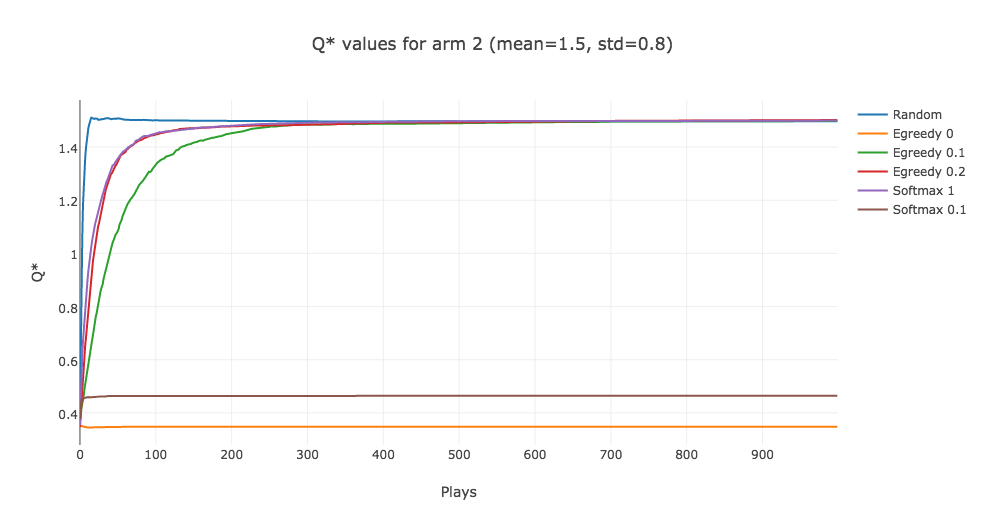
\includegraphics[width=0.7\textwidth]{img/1-2/q3.png}
\end{figure}


\begin{figure}[H]
   \centering
   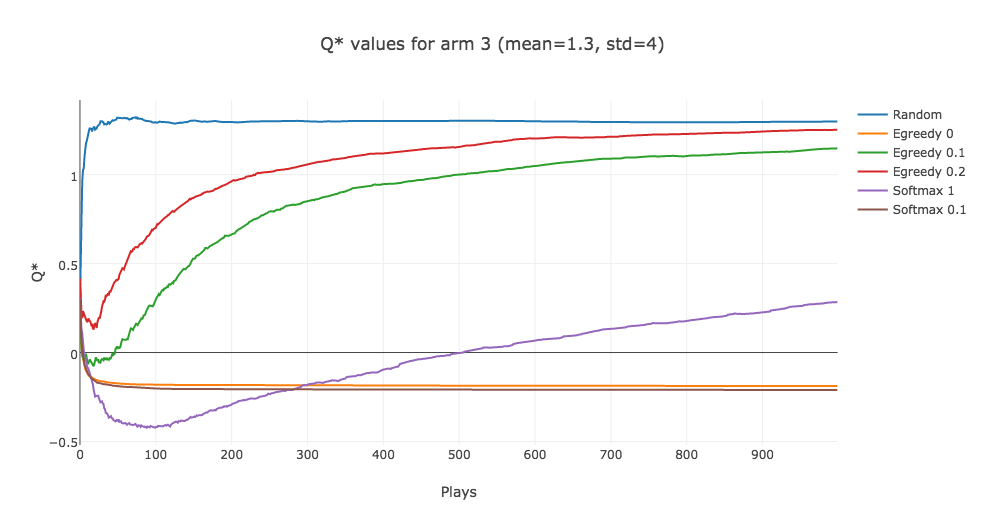
\includegraphics[width=0.7\textwidth]{img/1-2/q4.png}
\end{figure}


\subsubsection{Histogram}

\begin{figure}[H]
   \centering
   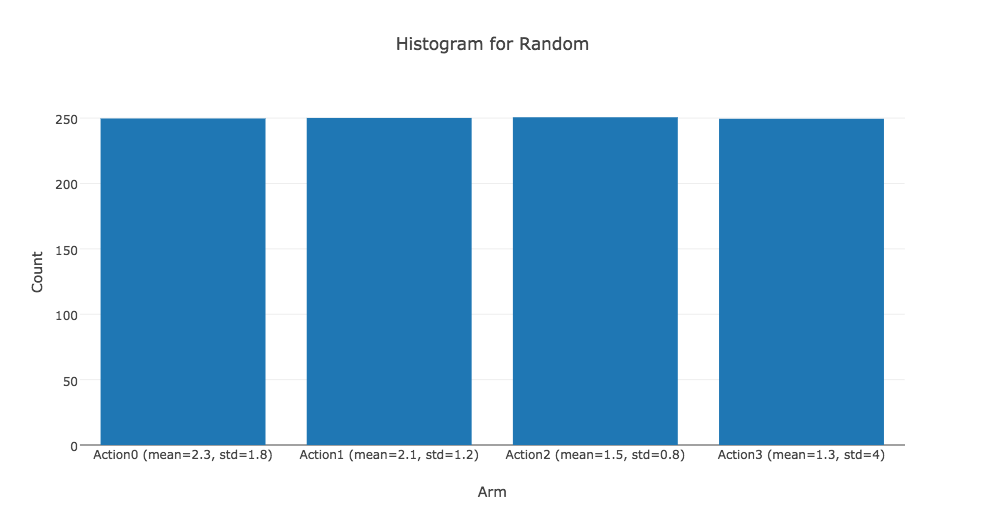
\includegraphics[width=0.7\textwidth]{img/1-2/h1.png}
\end{figure}

\begin{figure}[H]
   \centering
   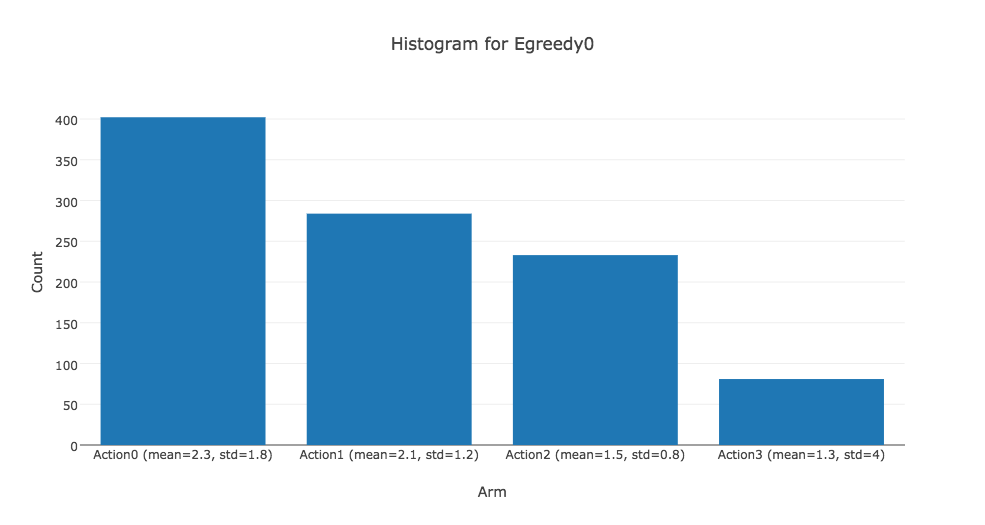
\includegraphics[width=0.7\textwidth]{img/1-2/h2.png}
\end{figure}

\begin{figure}[H]
   \centering
   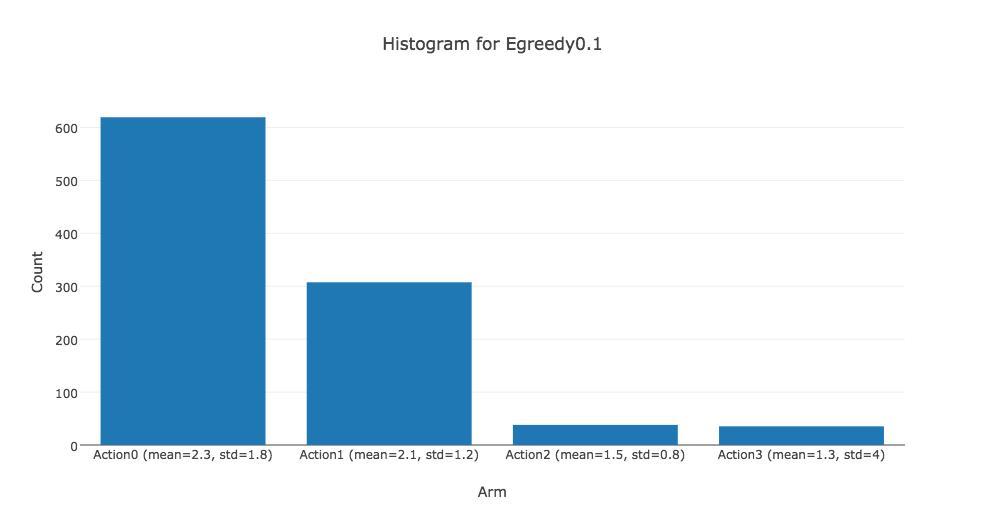
\includegraphics[width=0.7\textwidth]{img/1-2/h3.png}
\end{figure}

\begin{figure}[H]
   \centering
   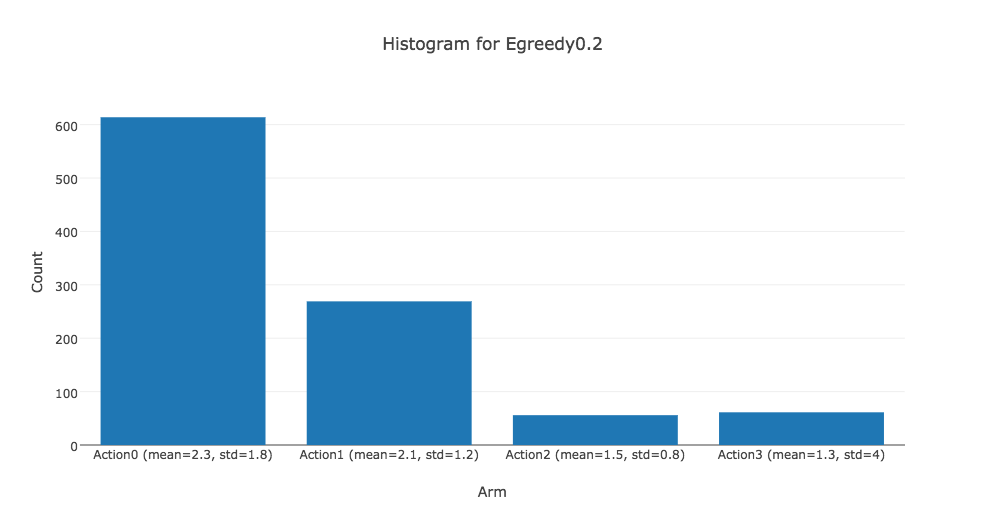
\includegraphics[width=0.7\textwidth]{img/1-2/h4.png}
\end{figure}

\begin{figure}[H]
   \centering
   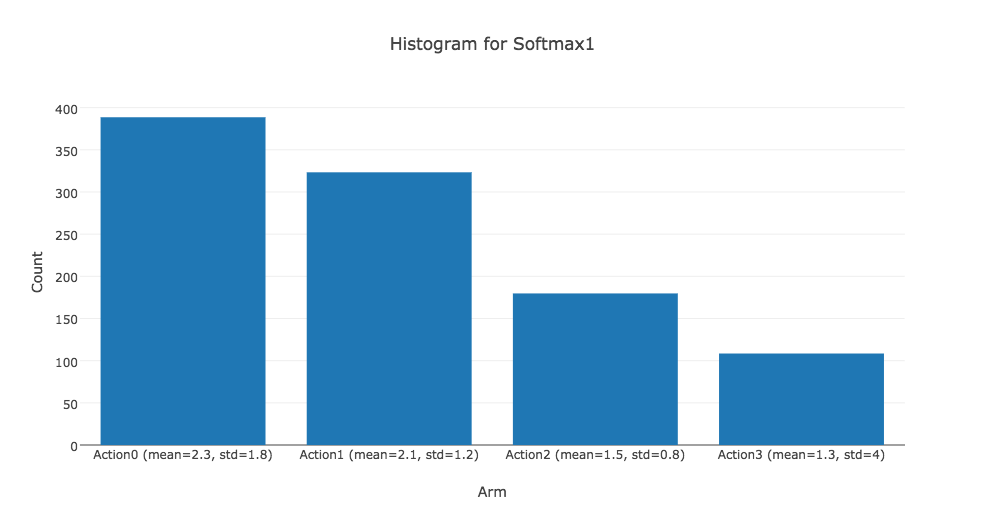
\includegraphics[width=0.7\textwidth]{img/1-2/h5.png}
\end{figure}

\begin{figure}[H]
   \centering
   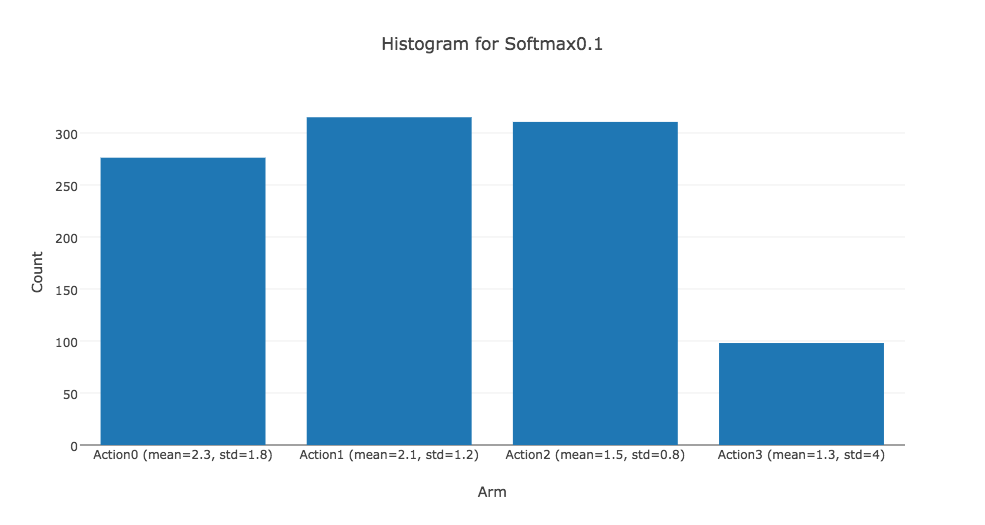
\includegraphics[width=0.7\textwidth]{img/1-2/h6.png}
\end{figure}


\subsubsection{Results}

\subsection{Exercice 3}


\subsubsection{Average reward for each algorithm}

\begin{figure}[H]
   \centering
   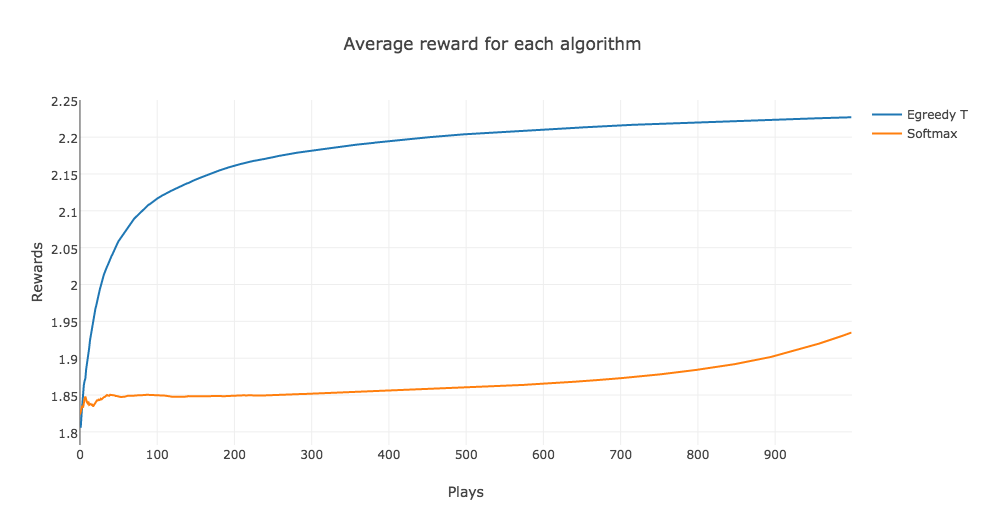
\includegraphics[width=0.8\textwidth]{img/1-3/reward.png}
\end{figure}

\subsubsection{Plot per arm}

\begin{figure}[H]
   \centering
   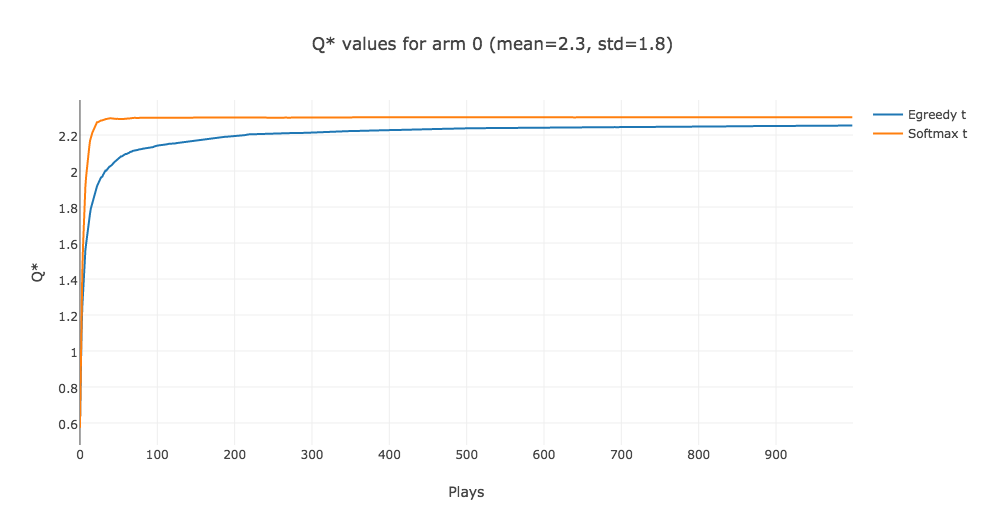
\includegraphics[width=0.7\textwidth]{img/1-3/q1.png}
\end{figure}

\begin{figure}[H]
   \centering
   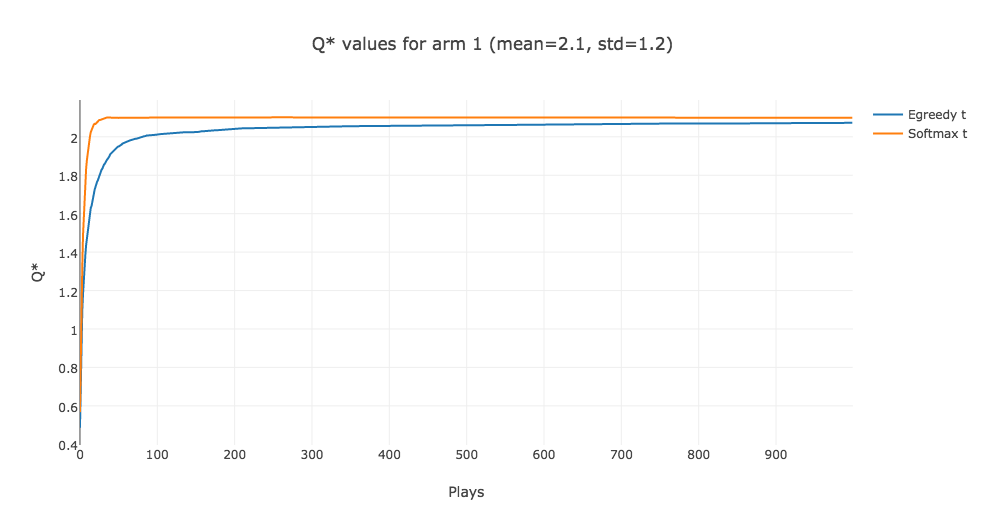
\includegraphics[width=0.7\textwidth]{img/1-3/q2.png}
\end{figure}

\begin{figure}[H]
   \centering
   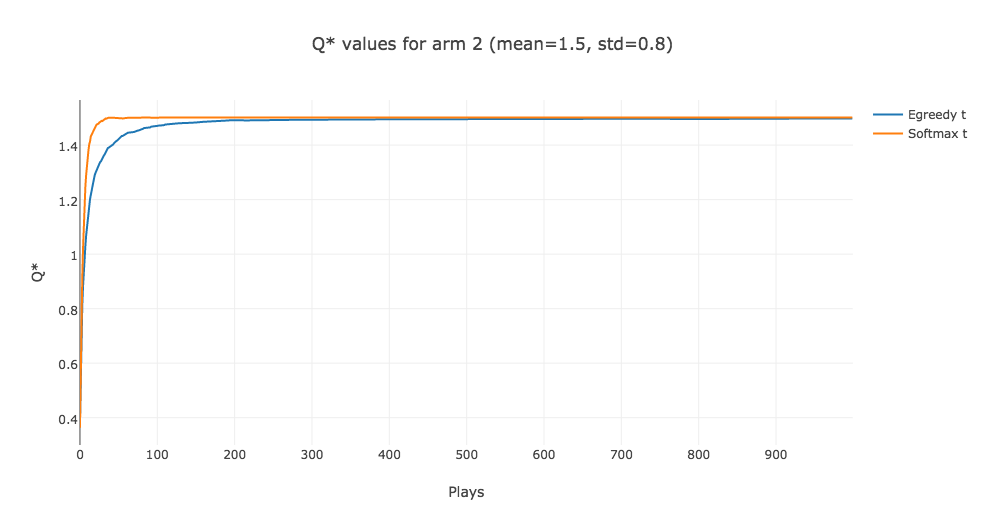
\includegraphics[width=0.7\textwidth]{img/1-3/q3.png}
\end{figure}


\begin{figure}[H]
   \centering
   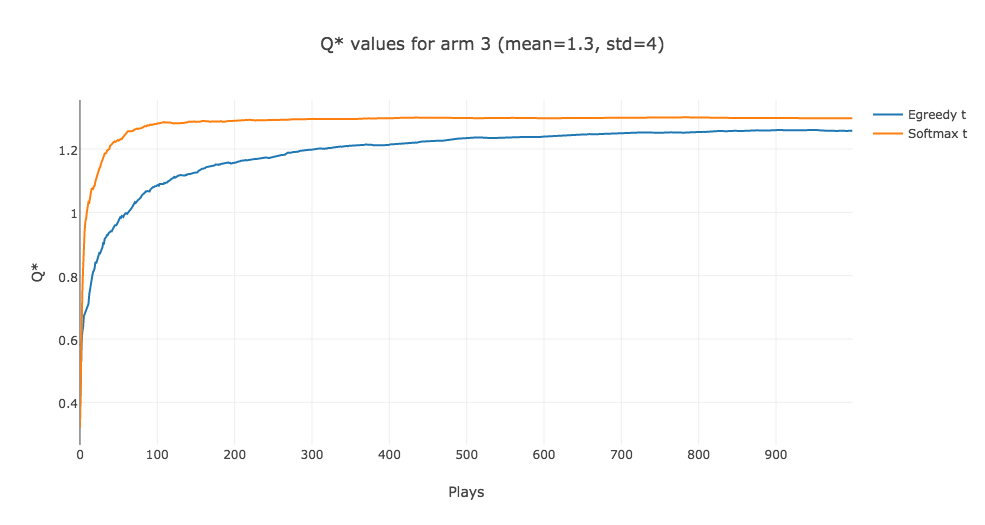
\includegraphics[width=0.7\textwidth]{img/1-3/q4.png}
\end{figure}


\subsubsection{Histogram}

\begin{figure}[H]
   \centering
   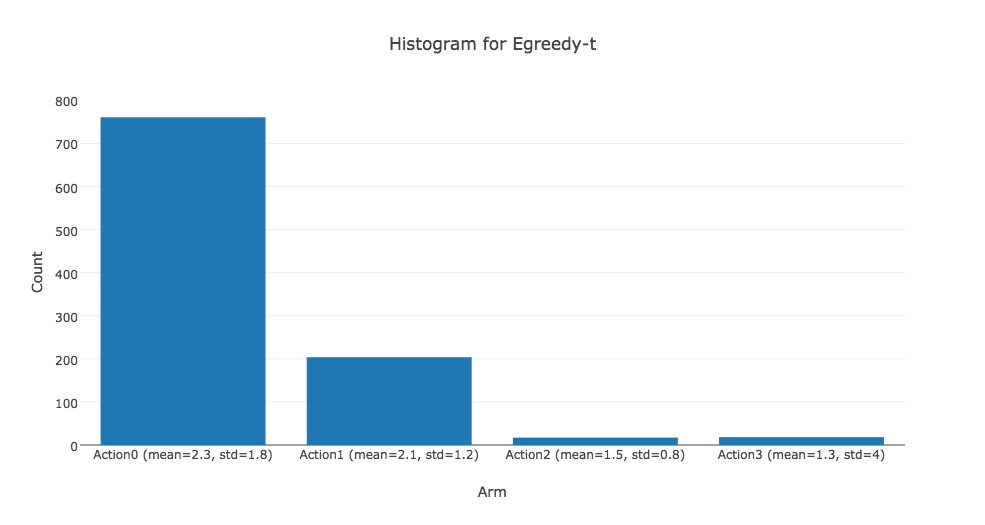
\includegraphics[width=0.7\textwidth]{img/1-3/h1.png}
\end{figure}

\begin{figure}[H]
   \centering
   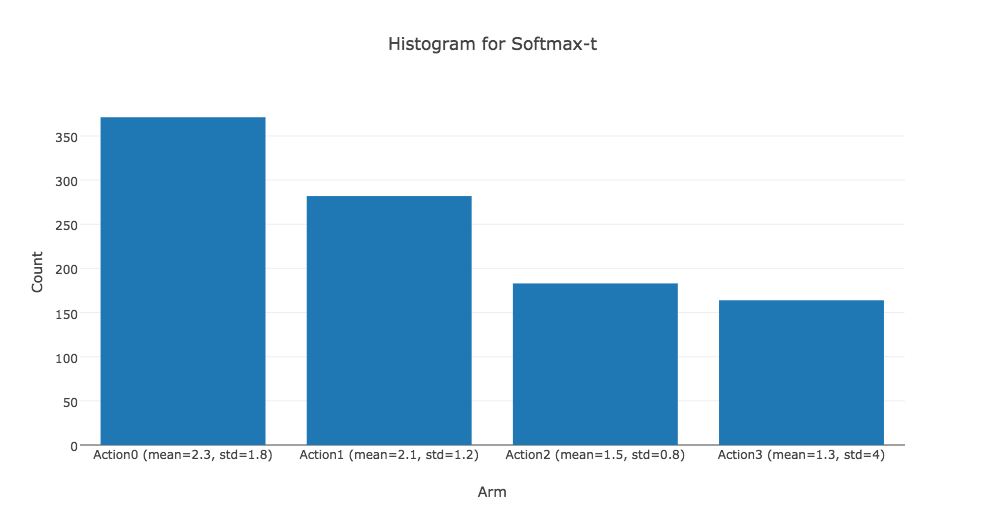
\includegraphics[width=0.7\textwidth]{img/1-3/h2.png}
\end{figure}


\subsubsection{Results}


\section{Stochastic Reward Game}

\end{document}







































              